\documentclass{scrartcl}

%\usepackage{etex}
\usepackage[left=3cm,right=2.0cm,top=1.25cm,bottom=1.75cm,includehead,includefoot]
{geometry}
\usepackage{marginnote}
\reversemarginpar
%Math
\usepackage{amsfonts,amsmath,amssymb,amsthm, amstext}
%Language, encoding, ...
\usepackage[utf8]{inputenc}
\usepackage[T1]{fontenc}
\usepackage[english]{babel}
\usepackage{t1enc, lmodern, textcomp}
%Pictures
\usepackage{graphicx, color}
%\usepackage{latexsym}
%\usepackage{keyval}
%\usepackage{ifthen}
%\usepackage{moreverb}
\usepackage[shell]{gnuplottex}
%Colors
\usepackage[usenames,dvipsnames]{xcolor}
\definecolor{darkblue}{rgb}{0.0, 0.2, 0.6}
\renewcommand*{\marginfont}{\bf\color{darkblue}}
%Nice a/b fractions
\usepackage{xfrac}
%Make it possible to write (fat) upright greek letters
\usepackage{upgreek}

%For indices
\newcommand{\ix}[1]{_{\mathrm{#1}}}
\newcommand{\Ix}[1]{^{\mathrm{#1}}}

%Directly include svg images
%%%%%%%%%%%%%%%%%%%%%%%%%%%%%%%%%%%%%%%%%%%%%%%%%%
\newcommand{\executeiffilenewer}[3]{%
    \ifnum\pdfstrcmp{\pdffilemoddate{#1}}%
    {\pdffilemoddate{#2}}>0%
    {\immediate\write18{#3}}\fi%
}
\newcommand{\includesvg}[1]{%
    \executeiffilenewer{#1.svg}{#1.pdf}%
    {inkscape -z -D --file=#1.svg %
    --export-pdf=#1.pdf --export-latex}%
    \input{#1.pdf_tex}%
}
%%%%%%%%%%%%%%%%%%%%%%%%%%%%%%%%%%%%%%%%%%%%%%%%%%

%Make captions look okay
\usepackage[font=small,format=plain,labelfont=bf,up,up]{caption}

%Hyperlinks
\usepackage{hyperref}
\hypersetup{
            pdflang=en-EN,
            unicode=true,
            pdfauthor={Thomas Staudt, Erik Schultheis},
}

%Differential d's
\newcommand{\dif}{\mathrm{d}}
\newcommand{\tdif}[2]{\ensuremath{\frac{\dif#1}{\dif#2}}}
\newcommand{\pdif}[2]{\ensuremath{\frac{\partial#1}{\partial#2}}}
\newcommand{\ppdif}[2]{\ensuremath{\frac{\partial^{2}#1}{\partial#2^{2}}}}
%Degree
\newcommand{\degr}{^\circ}

\renewcommand{\refname} {Literature}
\renewcommand{\figurename}{\bf Figure}
\newcommand{\fs}[1]{\footnotesize #1}
%double slash
\newcommand{\git}{\mathbin{
  \mathchoice{\textbackslash\mkern-6mu\textbackslash}% \displaystyle
    {\textbackslash\mkern-6mu\textbackslash}% \textstyle
    {\textbackslash\mkern-5mu\textbackslash}% \scriptstyle
    {\textbackslash\mkern-5mu\textbackslash}}}% \scriptscriptstyle


%Bibliography
\usepackage[babel]{csquotes}
\usepackage[backend=bibtex8]{biblatex}


\newcommand*{\defeq}{\mathrel{\vcenter{\baselineskip0.5ex \lineskiplimit0pt
                     \hbox{\scriptsize.}\hbox{\scriptsize.}}}%
                     =}



%\bibliography{sources}




\begin{document}

\begin{titlepage}\centering
\textsc{\Large Institute For Nonlinear Dynamics \\[1.5ex] Universität Göttingen}

\vspace*{2cm}
{\huge A Practical Course On Network Science}
\vspace*{2cm}

\rule{\textwidth}{1pt}\\[0.5cm]
{\bfseries \huge Block C: \\[0.5cm] \huge \bfseries Community and Structure\\[0.5cm]}
\rule{\textwidth}{1pt}

\vspace*{4cm}

\begin{Large}\begin{tabular}{rl}
        \textbf{Participants:}  & Erik Schultheis                                \\    
                   & \textit{erik.schultheis@stud.uni-goettingen.de}\\[0.5cm]
                   & Thomas Staudt                                  \\
                   & \textit{thomas.staudt@stud.uni-goettingen.de}  \\[1.0cm]

       \textbf{Tutors:}        & Xiaozhu Zhang, Nora Molkenthin, Benjamin Schäfer, \\
                               & Malte Schröder                                    \\[1.0cm]
       \textbf{Deadline:}      & 30.06.2015
\end{tabular}\end{Large}

\vspace*{1.5cm}


\end{titlepage}

\tableofcontents
\clearpage
\section{Communities in Networks}
When searching for (local) properties and ways of classifying networks, one
interesting aspect is the \emph{community structure} of the network in
question. That is, how can the network reasonably be divided into connected
components so that the nodes of the same component interact stronger than
the nodes of different components do (meaning that the components form
\enquote{communities}).

One way of obtaining the community structure of a network $G = (V,E)$ is by
disintegrating it (via removing edges) according to the edges' values of
the \emph{shortest path betweenness centrality} $g$. The betweenness
centrality $g(e)$ of an edge $e$ measures how \enquote{central} an edge is
for efficient connectivity in the network. More precisely it describes how
often $e$ is averagely used when taking the shortest path between two
nodes, thus
\begin{equation}\label{eq:betweenness}
    g(e) = \sum_{s,t\in V} \frac{\sigma(s,t | e)}{\sigma(s,t)}~,
\end{equation}
where $\sigma(s,t)$ is the number of shortest paths between the nodes $s$
and $t$ and $\sigma(s,t |e)$ is the number of those paths that go through
$e$. So edges with a high value of $g$ are likely to be important for
mediating between different communities of the graph.

Having obtained a breakdown of the network in connected subgraphs
(understood as communities) one must next be able to assess the quality and
strength of this community structure, e.g.\ for finding the optimal
number of communities. This can be done by calculating the
\emph{modularity} $Q(H)$ for a partitioning $H$ of the network $G$ (the
formula used to calculate $Q$ can be found on the respective handout for
C.1.1).
In the following, the variable $h$ will stand for the number of communities
for a given partitioning $H$ of a graph $G$.

Another property used to characterize given community structures is 
the stability $r(H, t)$ of the given division $H$ of $G$ in
partitions for different time scales $t$. This measure tells us how likely
it is to end up in the same community $c\in H$ that we started in, if
a random walk of length $t\in\mathbb{N}$ was carried out. Though the
stability could approximately be calculated by simulating random walks on
the graph, the analytic approach of the handout for C.1.2 was used for the
calculations below.


\subsection{The Karate Club Network}
The first network $G_0$ to be analyzed for its group structure was a given
network for a karate club. The original graph as well as the achieved
decompositions in communities for $h=2$ and $h=5$ are visualized in
\ref{fig:12_gr}.
Next the modularity of each community structure obtained for the different
numbers $h$ of communities was calculated. This modularity curve is
depicted in figure \ref{fig:12_mod} and shows that the found partitionings
with 2 and 5 communities are in fact the ones with the highest modularity
$Q$.

\subsection{Artificial Networks With Strong Community Structure}
Besides the karate network $G_0$ the same algorithms for community
detection and their modularity were used for other networks as well.
They are visualized -- together with selected decompositions -- in figure
\ref{fig:12_gr}.
\begin{itemize}
    \item [\textbf{$G_1$}] A simple deterministic network consisting of
        a triangle of center-nodes each connected to hexagons.
    \item [\textbf{$G_2$}] A more complex deterministic network consisting
        of 9 center-nodes each connected to 20-gons.
    \item [\textbf{$G_3$}] A random network with a grouping structure of
        $4\times 25$ nodes. Each node is connected to nodes in its own
        group with $p_g=0.75$ and to nodes in other groups with $p_o
        = 0.1$.
\end{itemize}

For each of these artificially community-structured networks the
algorithm based on the shortest-path betweenness centrality managed to find
the obvious community structures (as is depicted in figure
\ref{fig:12_gr}) and these obvious communities were indeed global
maxima of the modularity $Q$ when compared to the other communities
obtained (see figure \ref{fig:12_mod}).

As a side node, however, the algorithm failed to obtain the community
structure for $G_3$ if the difference between $p_g$ and $p_i$ was chosen
to be smaller. For $p_g = 0.65$ and $p_i = 0.15$ e.g.\ the desired
decomposition into four rings was not achieved.

\subsection{From Random Walks to Communities}
As the last task of this section, we calculated the stability curves
$t\mapsto r(H, t)$ of the four networks $G_0$, $G_1$, $G_2$, and $G_3$ for
different partitionings $H$ (obtained in the same way as above). The
resulting stability curves for time scales $1\le t \le 100$ can be seen in
figure \ref{fig:13}.

The results are as expected and show that the stability is in most cases
indeed best for the same communities that also exhibit the highest
modularity. For large time scales though, one can see for $G_2$ and $G_3$ that
partitionings with fewer communities than the expected value $h = 9$ and
$h=4$ are more stable. Since longer random walks cover longer distances 
this behaviour is not surprising.

\begin{figure}[bcht]
    \centering
    \gnuplotloadfile[terminal=epslatex, terminaloptions={color size 6.5,4.0}]{pictures/11.gp}
    \caption{Modularity curves of the networks $G_0$ (karate), $G_1, G_2,$
        and $G_3$ described in the text. For community structures
        corresponding to the vertical lines explicit visualizations may be
        found in figure \ref{fig:12_gr}.}
    \label{fig:12_mod}
\end{figure}


\begin{figure}
    \centering
    \def\svgwidth{0.8\textwidth}
    %\input{pictures/12.pdf_tex}
    \input{12.pdf_tex}
    \caption{Visualizations of the graphs $G_0$, $G_1$, $G_2$, and $G_3$
    before ($h = 1$) and after ($h > 1$) the algorithm for finding
    communities -- using the betweenness centrality -- has been applied,
    where $h$ denotes the number of communities in the respective
    partitioning $H$. For $G_0$ the colors were chosen based on the
    knowledge of the partitioning for $h=2$.  For $G_1$, $G_2$, and $G_3$
    the colors were chosen according to the obvious community
    structur we had in mind when creating these networks. All of these
    obvious structures were found by the algorithm: $h = 3$ for $G_1$,
    $h=9$ for $G_2$, $h=4$ for $G_4$.}
    \label{fig:12_gr}
\end{figure}


\begin{figure}
    \centering
    \gnuplotloadfile[terminal=epslatex, terminaloptions={color size 6.35,8.0}]{pictures/13.gp}
    \caption{Double-logarithmic plots of the stability curves for selected
    partitionings $H$ of the networks $G_0$ (karate), $G_1, G_2,$ and
    $G_3$ described in the text. The numbers $h_\mathrm{max}$ printed above
    the graphs correspond to the number of communities for which the
    stability was highest in the respective time scale interval.}
    \label{fig:13}
\end{figure}

\clearpage

\section{Network Motifs and Optimal Network Design}
\subsection{Motifs in Erdös-Renyi and Small-World Networks}
Until now we have looked at network structure only from a global
perspective (e.g by considering degree histograms, avg. shortest path
length etc.), but for real network applications much information can
probabily be found in more local structures. Therefore, we introduce the
notion of a network \emph{motif}. This is a connected subgraph that occurs often
enough in the given graph $G$ that it can be considered to be relevant.
One possible criterion for relevance is the comparison of occurances in the
investigated graph compared to a random graph that shares the global 
characteristics of the former, i.e. its nodes have the same degrees.

We define the relevance $r$ of a $k$-motif $M$ of a graph $G$ as the
precentage of $k$-node subgraphs $S_k$ of $G$ that are isomorphic to $M$,
i.e. where there exists a permutation of its nodes so that it is identical
to $M$. Let $\chi_M$ be that characteristic function of $M$, i.e.
$\chi_M(S) = 1$ iff $S$ is isomorphic to $M$. 
For finite graphs, $r$ can thus be calculated by 
\begin{align}
 r = (\# S_k)^{-1} \cdot \sum_{g \in S_k} \chi_M (g).
\end{align}
Since the number of possible $k-$node subgraphs grows exponentially fast,
evaluating this sum directly is not feasible for large graphs. Therefore,
we sample this sum (i.e. Monte-Carlo technique), where $p(g)$ denotes the
probability of chosing the sample $g$:
\begin{align}
 r \approx \frac{1}{N} \sum_{i=1}^{N} \frac{\chi_M (g_i)}{p(g_i)}.
\end{align}

We now focus our attention on $3$-motifs. Since $M$ is connected, we can
restrict sampling to connected subgraphs in the following way: 
\begin{enumerate}
\item choose a random starting node $A$ 
\item choose $B$ as a neighbour of $A$
\item choose $C$ as a common neighbour of $A$ and $B$. 
\end{enumerate}
The probability of taking this sample is ($N(k)$ denoting neighbours of $k$)
\begin{align}
 p(A,B,C) = \underbrace{1/N}_{A} \cdot \underbrace{1/\#N(A)}_{B} \cdot \underbrace{1/\#(N(A) \cap N(B))}_{C}.
\end{align}

If we assume that the graph in question is large enough, and that there is
no correlation between individual node degrees and the motifs, the
different values of $p(A,B,C)$ will average out, and we can disregard the
dependence to sampling probability. 

We assume this probability to hold for random directed Erdös-Renyi and
Watts-Strogatz graphs, for which we investigate the occurance of 3-motifs.
For ease of reference, we enumerate the motifs as shown in fig. \ref{fig:motifs}.
We consider graphs with average degree $8$ ($\left< k\ix{out} \right> = 5$, as required 
be the exercise, does not make sense for the Watts-Strogatz graph), the rewire
probability for Watts-Strogatz was chose to be $\SI{10}{\percent}$.

Since $p=4/99$ is low in the Erdös-Renyi network, we get sparse
connectivity, and thus motifs with less edges are more likely. Since there
are two possible realisations for motif $2$ compared to $1$ and $4$, $2$
has twice the probability, which is $\SI{45}{\percent}$. For motif $5$
another connection is required, so it is less probable by a factor
$p/(1-p) \cdot 3 = 0.12$ (the $3$ results from the $6$ total possible edge
direction distributions that result in this pattern, compared to the two
for pattern $2$), which gives $r_5=\SI{5.4}{\percent}$ in accordance with
the numerical findings. Pattern $11$ contains another additional edge, so it is
again less probable by a factor of order $0.1$.

Since Watts-Strogatz starts off with a ring structure that consists
entirely of the motifs 13 (neighbouring points) and 8 (if $C$ is not a direct
neighbour of $A$ and $B$), these patterns, and slight variations (i.e. 12,
7 and 3) thereof,  comprise the majority of motifs encountered in those graphs. We
find motif 2 with $\SI{5}{\percent}$ probability, $5$ with
$\SI{0}{\percent}$ and 11 with $\SI{1}{\percent}$, which means that those
structures are not significant motifs of Small-World networks compared to
random Erdös-Renyi networks.


\begin{figure}
	\centering
		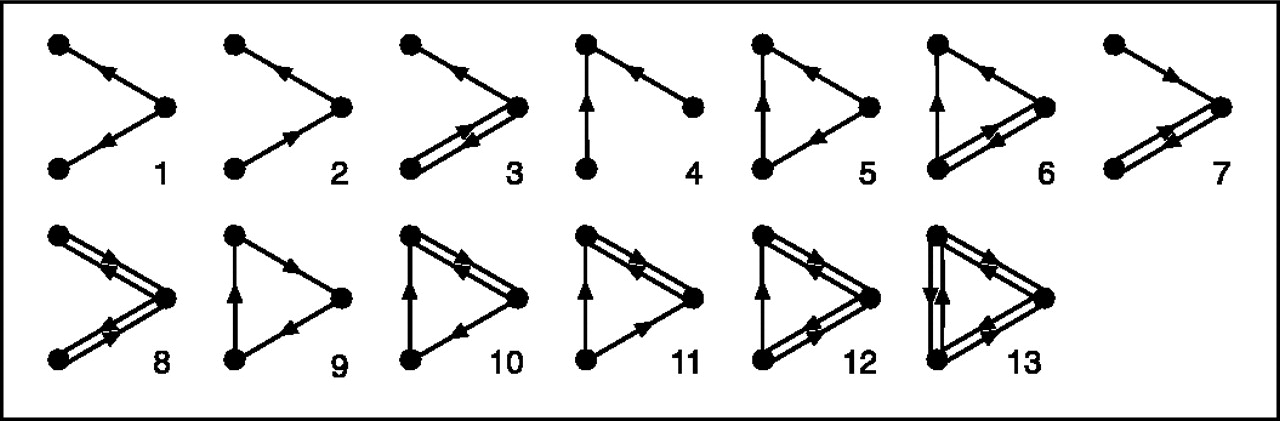
\includegraphics[width=1.00\textwidth]{pictures/motifs.png}
	\caption{All possible 3-motifs in directed graphs. Grpahic taken from {Milo et al (2002): Network Motifs: Simple Building Blocks of Complex Networks}}
	\label{fig:motifs}
\end{figure}

\begin{table}
	\centering
		\begin{tabular}{c|*{13}{r}}
		\toprule
		Motif & \num{1} & 2 & 3 & 4 & 5 &6 & 7 & 8 & 9 & 10 &11 & 12& 13  \\ \midrule
		Watts Strogatz & \num{2} & \num{5} & \num{15} & \num{2} & \num{0} & \num{1} & \num{15} & \num{25} & \num{0} & \num{1} & \num{1} & \num{12} & \num{21} \\
		Erdös Renyi & \num{22} & \num{45} & \num{2} & \num{22} & \num{5} & \num{0} & \num{2} & \num{0} & \num{2} & \num{0} & \num{0} & \num{0} & \num{0}\\
		\bottomrule
		\end{tabular}
	\caption{Relative percentual frequency of occurance of motifs in directed Watts-Strogatz and Erdös-Renyi networks. Motif numbers are taken from the presentation handout. The results were obtained by taking 10000 samples in 100 different, randomly generated networks of the designated topology. Each graph contained 100 nodes and the average degree was $k_{\mathrm{in}} = k_{\mathrm{out}}=4$, the rewire probability for Watts-Strogatz was chosen to be $\SI{10}{\percent}$.}
	\label{tab:motifs}
\end{table}

\subsection{Motifs in Real Networks}
A network describing hierarchical dependencies (e.g. predator-prey networks) will mostly contain the motifs 1 or 4, depending on the direction in which the relationsships are defined, as well as 2. Any motif containing bidirectional edges (3, 6-8, 10-13) or loops (9) will not appear. There might be situations in which structure 5 appears, e.g. omnivores that eat both plants and the animals that eat those.

A road network, on the other hand, will contain mostly bidirectional edges and therefore show mostly motifs 8 and 13. 

\subsection{Optimal Network Design}
For a given set of evenly and randomly spaced points on the unit square, we
want to determine the set of edges that constitute an optimal (in the sense
of optimizing both construction/maintenance cost as well as minimizing
travel times) transportation network.

We approximate the maintenance cost of the network as proportional to the
total edge length. For travel times, we take into account both the actual
time en route as well as possible mandatory delays at each stop, weighted
against each other with a factor $\delta$. The total network cost function
is then a weighted sum of both terms, with a weight of $\alpha$ to relate
them.  

Also included is scaling factor of $\sqrt{N}$ such that the maintenance and
the travel cost obtain the same scaling with $N$. The final cost formula
thus is
\begin{align}
 K = \alpha \sum_{i,j} r_{ij} A_{ij} + \left< l \right>,
\end{align}, where $r_{ij}$ denotes the geographical distance between the points $i$ and $j$, $A_{ij}$ is the adjacency matrix.
The path length between two connected points is 
\begin{align}
 l_ij = (1-\delta) \sqrt{N} r_{ij} + \delta.
\end{align}
 
Finding the network for which $K$ is minimized is next to impossible,
because we are operating on a vast, discrete state space where the function
$K$ has many local minima. This means that neither methods based on
jacobians or gradient descent nor an exhaustive search are feasible. 
An algorithms specifically designed to takle these kind of problems is
\emph{Simulated Annealing}, which performs a random walk through the state space,
that has the possibility to reject a step if the resulting cost function
would be higher. The acceptance probability or worse states is inspired by thermodynamics
and chosen to be $\exp \Delta K/T$, where the "temperature" $T$ is
decreased over the course of the algorithm to tune it from exploration to
minimization. The possibility to go to a worse state prevents the algorithm
from getting stuck in a local minimum early on.

Applying the method to a network of $25$ locations with a value of
$\alpha=0.1$ and $\delta \in \{0, 0.5, 1\}$, ($T$ was chosen to be 0.01
intially and was decreased by factor 0.99 in each of the 1000 cooling steps.
This parameter, however, is not relevant for the model, but affects the
performance of the annealing and thus the quality of the soution found.)
results in the optimized networks shown in figure \ref{fig:motifs}. For
$\delta=0$, it resembles a road network, as switching roads is essentially
free, whereas $\delta=1$ looks like airplane routes, because waiting times
at airports can constitute a significant amount of the travel time, so one 
central node conneted to many others becomes more attractive to the algorithm.
The result is not a perfect star topology, because the algorithm only finds
an approximative solution.

\begin{figure}[htbp]
\centering
\begin{minipage}[b]{.45\linewidth}
	\centering
	$\delta = 0$
	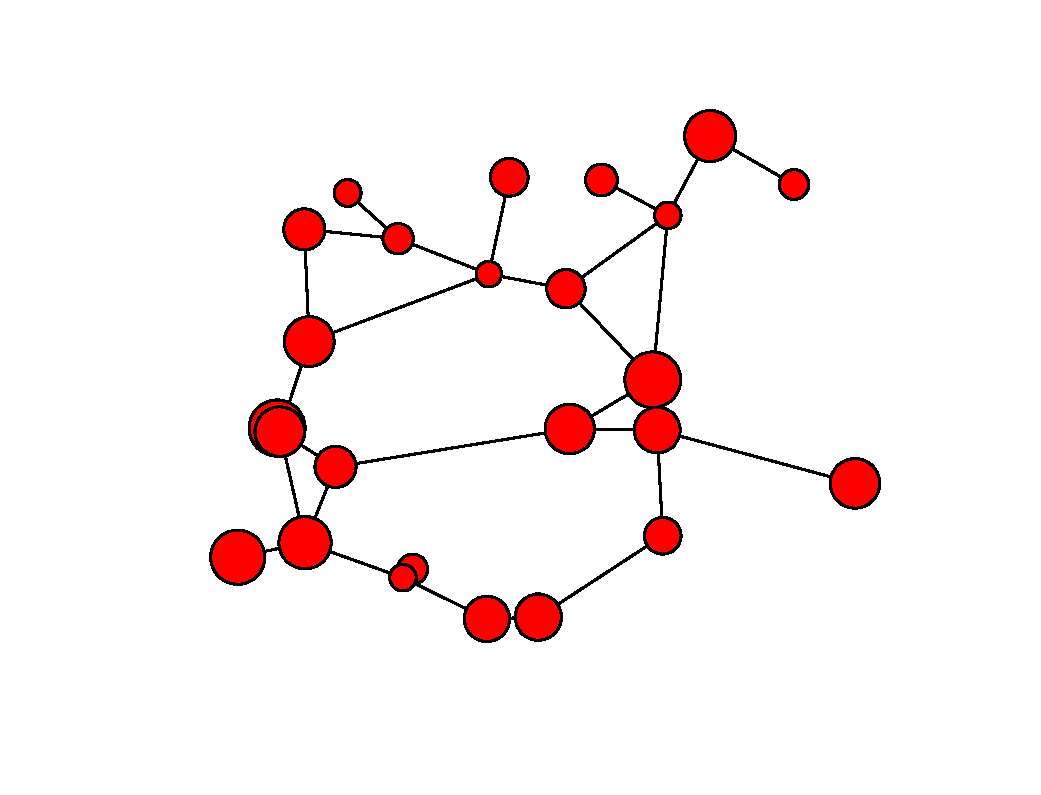
\includegraphics[width=\textwidth]{pictures/d0.pdf}
	\end{minipage}
	\nolinebreak 
	\begin{minipage}[b]{.45\linewidth}
	\centering
	$\delta = 0.5$
	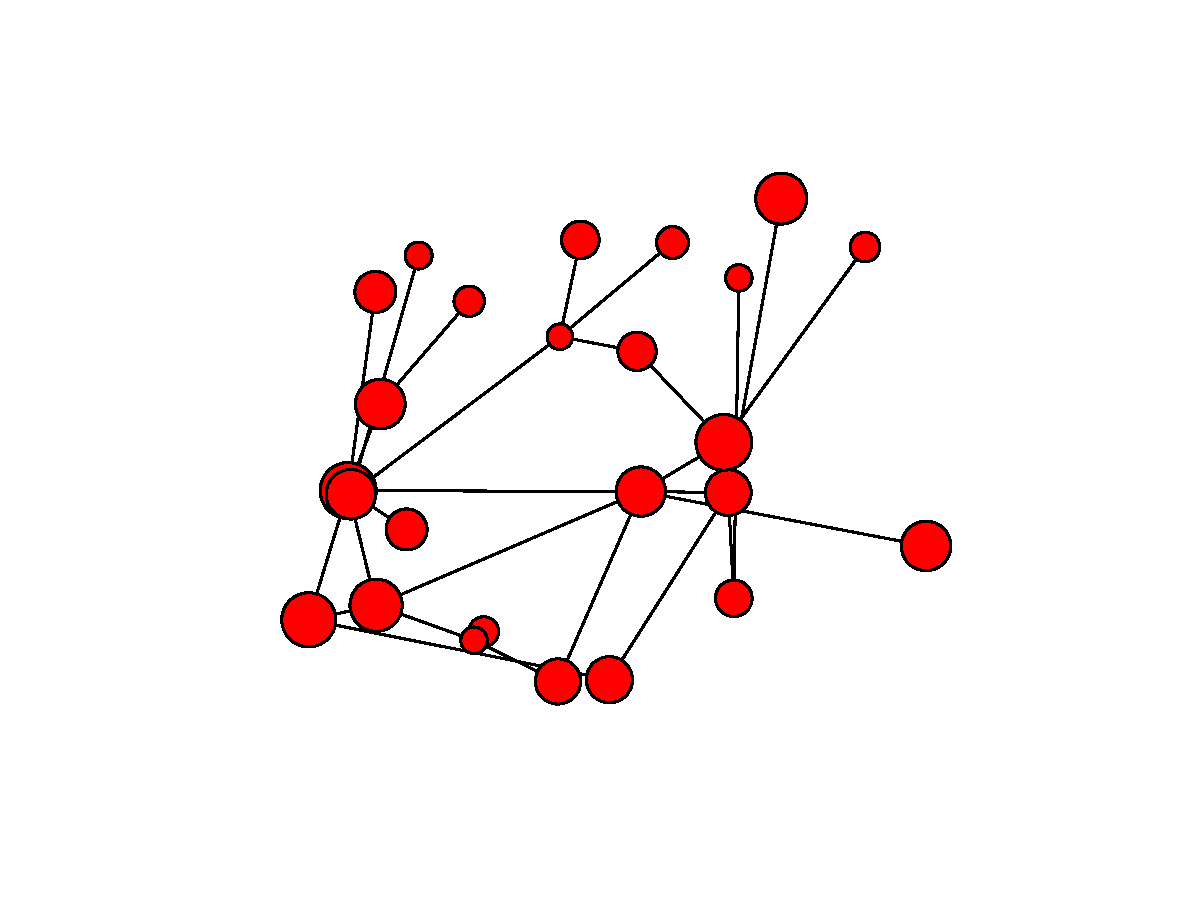
\includegraphics[width=\textwidth]{pictures/d5.pdf}
  \end{minipage}
	\begin{minipage}[b]{.45\linewidth}
	\centering
	$\delta = 1$
	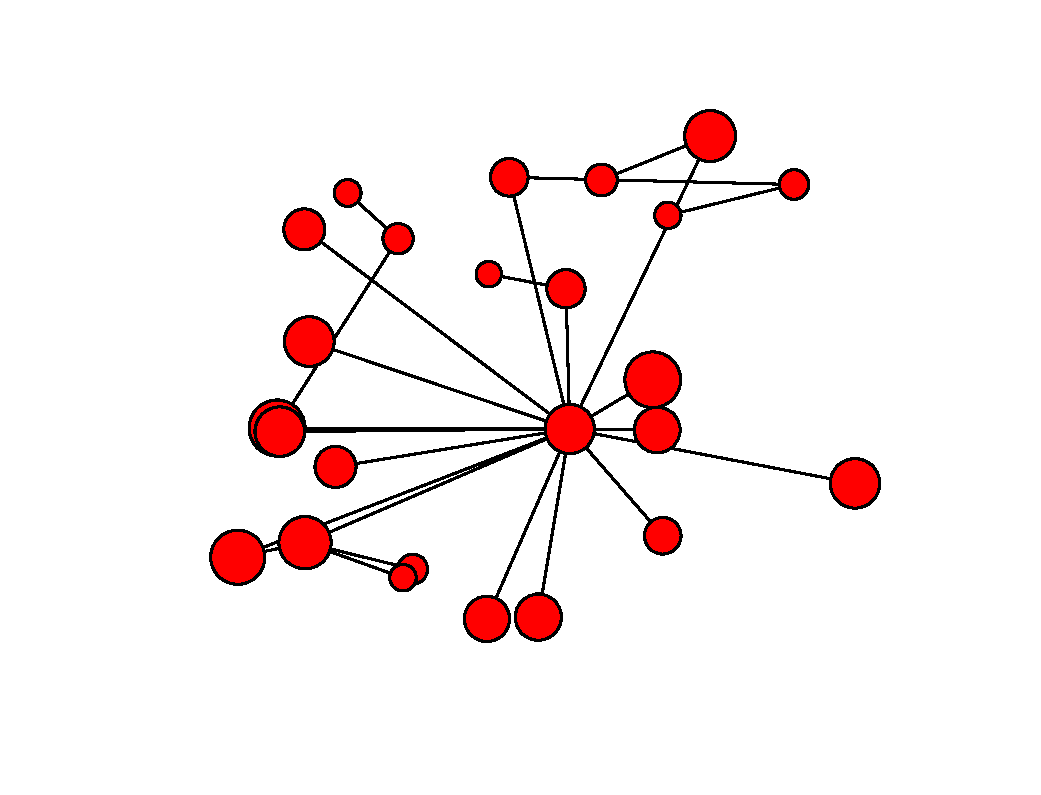
\includegraphics[width=\textwidth]{pictures/d10.pdf}
	\end{minipage} \nolinebreak
	\begin{minipage}[b]{.45\linewidth}
	\centering
	European Airports
	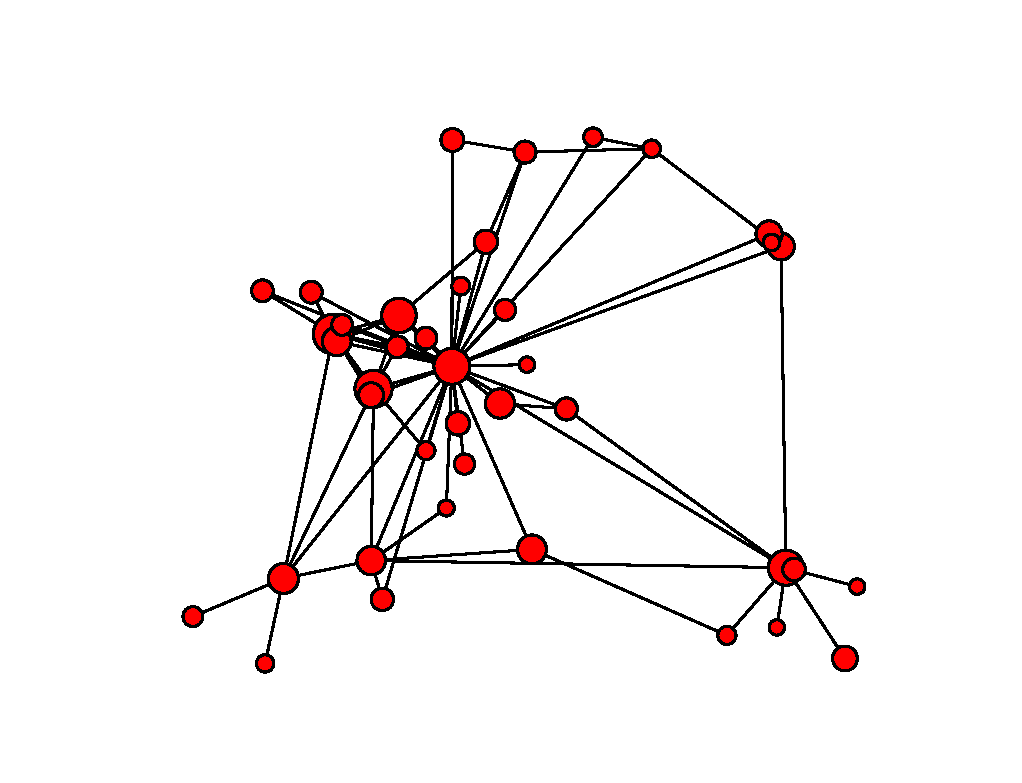
\includegraphics[width=\textwidth]{pictures/europe.pdf}
	\end{minipage}
	\caption{Network structure for $25$ random points in the unit square, optimized for $\delta \in \{0, 0.5, 1\}$, and for a network where the node positions were taken as the locations of the 40 busiest european for $\delta = 0.5$. }
	\label{fig:motifs}
\end{figure}


\clearpage 

\section{Search and Traffic on Networks}
For this section our interest lies on networks with nodes that are
understood as persons in a social graph. In this situation, a \emph{social
distance} between two persons can be implemented by comparing how
\enquote{near} these persons are in different social categories
(Are they in the same sports clubs or classes? Do they have similar hobbies
and music preferences?). 

As an application one can use the social distance
to implement a message passing system that works by iteratively relaying
the message to persons that have the same or similar social characteristics
as the target person.

\subsection{Creating Artificial Social Networks}
\subsection{Decomposing Artifical Social Networks}
\subsection{Message Passing}
\subsection{Relevance of Certain Nodes for Message Passing}


\begin{figure}
    \centering
    \def\svgwidth{0.9\textwidth}
    \input{311.pdf_tex}
    \caption{The generated social graphs for $S=1$ and \textbf{(a)} $\alpha = 1$
    as well as \textbf{(b)} $\alpha = 5$. The other parameters were $g = 5,
    l = 3$, and $k = 4$. The colors represent the different
    social groups that are given by the single characteristic $s$ to be
    used.  The two topmost graphs (\enquote{original}) are the full
    networks containing all edges, whereas the middle ($h = 4$) and
    lowermost ($h=8$) graphs represent the community structure derived by
    the decomposition algorithm of C1 when dividing the graph in
    4 respectively 8 communities.
    The layout was calculated anew for each plot so that the resulting
    communities can be discerned easily.}
    \label{fig:331}
\end{figure}

\begin{figure}
    \centering
    \def\svgwidth{0.9\textwidth}
    \input{312.pdf_tex}
    \caption{The generated social graphs for $S=2$ and \textbf{(a)} $\alpha
    = 1$ as well as \textbf{(b)} $\alpha = 5$. The other parameters were 
    $g = 5, l = 3$, and $k = 4$. The two characteristics of
    the social graphs are represented by colors and numbers (between 0 and
    7).  As in figure \ref{fig:331}, the two topmost graphs correspond to
    the full networks, while the other graphs correspond to decompositions
    in $h = 4$ and $h = 8$ communities, using the algorithm introduced in C1.
    Again, the positions of the nodes were chosen to be variable so that
    the community structures can be seen esier.}
    \label{fig:332}
\end{figure}


\begin{figure}[bcht]
    \centering
    \gnuplotloadfile[terminal=epslatex, terminaloptions={color size 6.5,4.0}]{pictures/33.gp}
    \caption{Relative frequencies of the path lengths that occur when
        transferring messages between persons with a shortest path of
        length $d$ between them. To obtain the data, $50$ social graphs
        with parameters $g = 5, l = 3, k = 4, s = 2, \alpha = 1$ were
        created and were then used to conduct $200$ message transferes each
        for $d\in\{1, 2, 3, 4\}$.  Only graphs with a maximum shortest path
        length of 4 or more (which happened very seldomly) were used. }
    \label{fig:12_mod}
\end{figure}


\end{document}

